\documentclass[british,english,aspectratio=169]{beamer}
\setbeamertemplate{caption}{\raggedright\insertcaption\par}
\setbeamerfont{caption}{size=\footnotesize}
\usepackage{tikz}
\usetikzlibrary{positioning}
\usepackage{smartdiagram}
\usepackage{caption} % Load the caption package
\usepackage{annotate-equations} 
\usepackage{colortbl}
\definecolor{LightNavyBlue}{cmyk}{0.6, 0.3, 0, 0.1}
\definecolor{LightGreen}{cmyk}{0.6, 0.3, 0.6, 0.1}
\definecolor{Plum}{cmyk}{0.50, 1.0, 0, 0.4} 
\usepackage{fontawesome5}
\usepackage{nicefrac}
\usepackage{xcolor}
\definecolor{royalblue}{RGB}{65,105,225}


\captionsetup{labelformat=empty}

\usepackage{graphicx} 

\usetheme{Boadilla}
\usecolortheme{orchid}
\title[EAGLE with individual countries]{The EAGLE model with individual euro area countries: a framework for fiscal policy analysis}
\author[K. Ba\'nkowski, E. Petravičiūtė]{Krzysztof Ba\'nkowski \and Emilė Petravičiūtė}
%//TODO: Put special signs in the names
\institute[] % (optional)
{
  Fiscal Policies Division\\
  European Central Bank
}


\date[June 2025] % (optional)
{Public Finance Workshop in Tallinn \\ 18 June 2025}

% Set the outer theme and options for the navigation bar
\useoutertheme[footline=empty,subsection=false]{miniframes}
% Set the inner theme
\useinnertheme{circles}
% Remove default navigation symbols
\setbeamertemplate{navigation symbols}{}

\begin{document}
\frame{\titlepage}
%Highlighting text

% Outline Slide
% \begin{frame}{Outline}
%   \tableofcontents
% \end{frame}

\section{Introduction}

\begin{frame}
  \frametitle{How much euro area countries trade}

  \begin{figure}
    \centering
    \includegraphics[width=0.95\textwidth, height=0.75\textheight]{figures/importMagnitude.png}
    \caption{\scriptsize Source: Own calculations based on World Integrated Trade Solution data}
    %TODO: if we have time, add source and adjust the size
  \end{figure}
\end{frame}

\begin{frame}
  \frametitle{The EAGLE model with individual countries}
  \vspace{-1ex}
  \begin{itemize}
  \item The original EAGLE model is a DSGE model representing the global economy as interconnected open economies, with 4 regions: Germany, rest of Euro Area, the US, and Rest of World, and portrays a shared monetary policy for euro countries. 
  \item The model embeds meaningful fiscal policy (notably, complementary government consumption and productive government investment), which makes it a suitable tool to analyse fiscal initiatives.
  \item We recognize the importance of heterogeneity and silmutaneous interdependence in the euro area.
  \item Against this background, we establish a more country-granular version with 10 EA countries and add a non-EA area EU region, making it in total a 14 region model. 
  \item This presentation focuses on trade extension, properties of main fiscal shocks, and the study of the Next Generation EU (NGEU) programme in our setup as a policy application.
  \end{itemize}
  \end{frame}


\section{Literature \& contribution of the project}
\begin{frame}
  \frametitle{Related literature \& Contribution}
  \textbf{Related Literature}
  \begin{itemize}
  \item Multitude of papers documenting and applying \textcolor{royalblue}{EAGLE} by Pascal Jacquinot and members of EAGLE network.
  \item Variety of applications of \textcolor{royalblue}{QUEST} model by colleagues from the EC.
  \item \textcolor{royalblue}{ECB-MC} already exists in the form of a linked version at the ECB.
  \item Other models like \textcolor{royalblue}{GIMF} at the IMF documented in Kumhof et al. (2010).
  \end{itemize}
  \textbf{Our Contribution}
  \begin{itemize}
  \item The 4 region EAGLE model can be calibrated for any EA country, but it does so only relating the country to EA as a whole, not grasping the heterogeneity within EA, and so is unsuited for multiple country fiscal programmes such as the NGEU programme, or defence spending. 
  \item We present a more granular version of the model operating in Dynare, equiped to analyse granular spill-over effects across Euro Area. 
  \end{itemize}
  \end{frame}


\section{Model specification}

\begin{frame}
  \frametitle{Final goods in the model}
  \begin{itemize}
  \item The model includes four final goods: private consumption, private investment, government consumption, and government investment.
  \item Final goods are assembled by perfectly competitive firms using intermediate inputs.
  \item Intermediate goods come from monopolistically competitive sectors: tradable (e.g. manufacturing) and non-tradable (e.g. services).
   \item Tradable goods can be imported and each good has a home-bias parameter. For example, government purchases have a higher home-bias parameter and use more of domestically produced goods.
   \item The model's multi-country trade structure and calibration of import content, which varies throughout the four goods for each region are key contributions.
  \end{itemize}
\end{frame}

\begin{frame}[t]
  \frametitle{Final goods in the model}
  \centering

  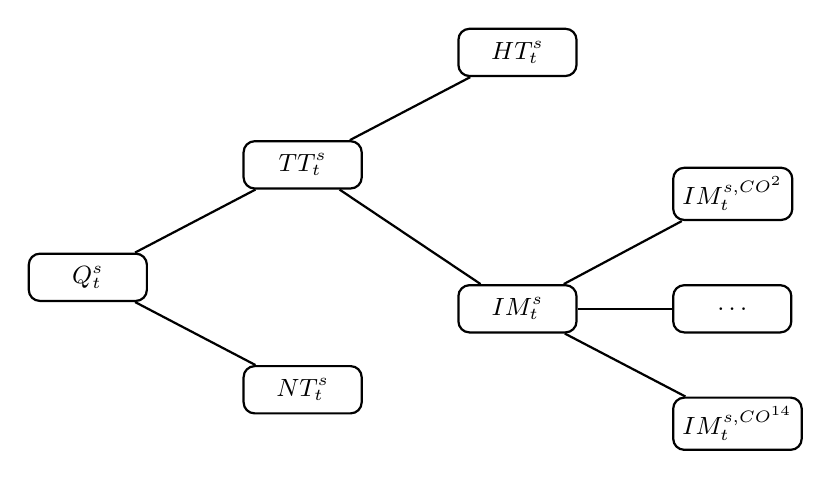
\begin{tikzpicture}[
    node distance=0.8cm and 1.2cm,
    every node/.style={draw, rounded corners, minimum width=1.5cm, minimum height=0.6cm, align=center, font=\small},
    every path/.style={draw, thick}
  ]
    \node (qt) {$Q_t^s$};
    \node[above right=of qt] (tt) {$TT_t^s$};
    \node[below right=of qt] (nt) {$NT_t^s$};
    \node[above right=of tt] (ht) {$HT_t^s$};
    \node[below right=of tt, yshift=-0.4cm] (im) {$IM_t^s$};
    \node[above right=of im] (im_CO1) {$IM_t^{s,CO^2}$};
    \node[right=of im] (im_CO2) {$\dots$};
    \node[below right=of im] (im_CO3) {$IM_t^{s,CO^{14}}$};

    \draw (qt) -- (tt);
    \draw (qt) -- (nt);
    \draw (tt) -- (ht);
    \draw (tt) -- (im);
    \draw (im) -- (im_CO1);
    \draw (im) -- (im_CO2);
    \draw (im) -- (im_CO3);
  \end{tikzpicture}

  \vspace{4mm}
{\scriptsize
  \textit{Note:} $Q_t^s$ = final good; $TT_t^s$ = tradable component; $NT_t^s$ = non-tradable component; $HT_t^s$ = home tradable good; $IM_t^s$ = imported tradable good; $IM_t^{s,CO^2}$, $IM_t^{s,CO^{14}}$ = imports from countries $CO^2$ and $CO^{14}$.
}
\end{frame}

\begin{frame}
  \frametitle{How do imported goods enter the model?}
  \centering
  \begin{figure}
  \includegraphics[width=\linewidth]{figures/eagle_chart3.png}
  \caption{\scriptsize Source: Own illustration.}
  \end{figure}
  \end{frame}

  \begin{frame}
    \frametitle{What are the trade aggregators?}
    \begin{itemize}
    \item \faBoxes~Tradable goods: % Changed from \faLandmark to \faBoxes to represent tradable goods
    \begin{equation*}
    TT_t^C(x)=\left[\eqnmarkbox[Plum]{p3}{v_{TC}}^{\frac{1}{\mu_{TC}}} \eqnmarkbox[LightNavyBlue]{p1}{HT_t^C(x)}^{\frac{\mu_{TC}-1}{\mu_{TC}}}+\left(1-v_{TC}\right)^{\frac{1}{\mu_{TC}}} \eqnmarkbox[LightGreen]{p2}{IM_t^C(x)}^{\frac{\mu_{TC}-1}{\mu_{TC}}}\right]^{\frac{\mu_{TC}}{\mu_{TC-1}}}
    \end{equation*}
    \annotate[yshift=-0.5em]{below,right}{p1}{Home tradables}
    \annotate[yshift=-0.5em]{below,right}{p2}{Imported goods}
    \annotate[yshift=-0.5em]{below,left}{p3}{Home bias parameter}
    \item \faShip~Imported goods: % Changed from \faLandmark to \faShip to represent imports
    {\small
    \begin{equation*}
    IM_t^C(x)=\left[\sum_{CO \neq H}\left(\eqnmarkbox[Plum]{p4}{v_{IM^C}^{H,CO}}\right)^{\frac{1}{\mu_{IMC}}}\left(\eqnmarkbox[LightGreen]{p5}{IM_t^{C,CO}(x)}\left(1-\Gamma_{IM^C}^{H,CO}\left(\frac{IM_t^{C,CO}(x)}{Q_t^C(x)}\right)\right)\right)^{\frac{\mu_{IMC}-1}{\mu_{IMC}}}\right]^{\frac{\mu_{IMC}}{\mu_{IMC}-1}}
    \end{equation*}
    }
    \annotate[yshift=-1.5em]{below,left}{p4}{Bias towards CO country}
    \annotate[yshift=-1.5em]{below,right}{p5}{Imported goods from CO country}
    \end{itemize}
    \end{frame}

\begin{frame}
  \frametitle{Trade and net foregin asset position}
\begin{itemize}
  \item Each country may run a trade surplus or deficit: exports and imports can differ in value.
  \item The nominal trade balance is defined as:
\end{itemize}

\vspace{2mm}
\begin{equation*}
  TB_t \equiv \sum_{CO \neq H} S_t^{H,CO} P_{X,t}^{H,CO} \underbrace{\frac{s^{CO}}{s^H} IM_t^{CO,H}}_{\equiv X_t^{H,CO}} - \sum_{CO \neq H} P_{IM,t}^{H,CO} IM_t^{H,CO}
\end{equation*}

\vspace{2mm}
\begin{itemize}
  \item $X_t^{H,CO}$: Exports from $H$ to $CO$, defined as $CO$'s imports from $H$ adjusted by the size ratio $\left(\frac{s^{CO}}{s^H}\right)$. $S_t^{H,CO}$ is the nominal exchange rate converting prices from $CO$'s to $H$'s currency.
  \item This scaling reflects how small economies can be heavily affected by trade with large partners.
  \item Important for steady-state calibration when countries differ significantly in size.
  \item Trade imbalances between countries are reflected in their net foreign asset (NFA) positions,
which materialize through international bond holdings.
\end{itemize}
\end{frame}

\begin{frame}{Fiscal and Monetary Policy rules}
\begin{itemize}
  \item Governments are not required to balance the budget in each period with the possibility of issue bonds. 
  \item Following Clancy et al. (2016) EAGLE extension, government consumption exhibits complementarity with private consumption, and government investment contributes to the stock of productive capital.
  \item For all fiscal instruments, except for lump-sum taxes, we assume a fiscal rule, whereby the fiscal instrument in year t is determined by the calibrated long-run target, smoothing parameter, and an i.i.d. shock to the instrument. 
  \item The fiscal rule governing lump-sum taxes is designed to ensure that government debt converges towards a long-run target level. Stability of the debt stock is
achieved through a gradual adjustment of lump-sum taxes relative to output.
  \item Central banks follow a Taylor-type interest rate rule, specified in terms of annual CPI inflation, and quarterly
output growth.
\end{itemize}
\end{frame}

\section{Model calibration}

\begin{frame}
  \frametitle{Import content of final demand components}
  \framesubtitle{Following the methodology of Bussière et al. (2013)}
  \begin{figure}
  \centering
  \includegraphics[width=0.9\textwidth]{figures/import_content2.png}
  \caption{\scriptsize Source: Own calculations based on the Eurostat Input-Output annual data.}
  \end{figure}
\end{frame}

\begin{frame}
  \frametitle{Import structure in EAGLE}
  \framesubtitle{Example for Spain}
  \vspace{-3ex}  % Added negative vertical space
  \begin{figure}
  \includegraphics[width=\textwidth, height=0.75\textheight]{figures/trade_values.png}
  \vspace{-9ex}  % Added negative vertical space
  \caption{\scriptsize Note: The numbers in grey are parameter values in trade aggregators. Otherwise, the figures are GDP shares of relevant components.}
  \end{figure}
  \end{frame}

\section[Model properties]{Model properties}


\begin{frame}
  \frametitle{EA-wide fiscal stimulus}
  \framesubtitle{1\% of ex-ante GDP fiscal expansion during 4 quarters in all euro area countries}
  \vspace{1ex}  % Added negative positive space
  \begin{figure}
  \centering
  \includegraphics[]{figures/effectGovEA.png} % Ensure the image fits the slide
  \caption{\scriptsize Note: The GDP values are in percentage deviation from the steady state. Inflation values are absolute deviations in percentage points.}
  \end{figure}
  \end{frame}

\begin{frame}
  \frametitle{National fiscal stimulus}
  \framesubtitle{1\% of ex-ante GDP fiscal expansion during 4 quarters in Spain only}

  \vspace{1ex}  % Added negative positive space
  \begin{figure}
    \centering
    \includegraphics[]{figures/effectGovES.png} % Ensure the image fits the slide
    \caption{\scriptsize Note: The GDP values are in percentage deviation from the steady state. Inflation values are absolute deviations in percentage points.}
  \end{figure}

\end{frame}

\section[Policy application]{NGEU eveluation}
  
\begin{frame}
  \captionsetup{font=scriptsize,justification=raggedright,singlelinecheck=off}
  \frametitle{NGEU-financed investment in the euro area}
  \framesubtitle{\% of the euro area GDP}
  \vspace{1ex}  % Added negative positive space


  \begin{figure}
  \centering
  \includegraphics[width=0.85\textwidth]{figures/NGEU_input.png}
  \vspace{-2ex}  % Added negative positive space
  \caption{Source: Own calculations based on the ESCB WGPF data.}  % Added caption
  \end{figure}
  \end{frame}

  \begin{frame}
    \captionsetup{font=scriptsize,justification=raggedright,singlelinecheck=off}
    \frametitle{The estimated overall NGEU effect}
    \vspace{1ex}  % Added negative vertical space to reduce gap
    \begin{figure}
    \centering
    \includegraphics[]{figures/effectNGEUtotal.png} % Ensure the image fits the slide
    \caption{\scriptsize Note: The GDP values are expressed as a percentage deviation from the baseline values. The inflation rate is an absolute deviation in percentage points.}
    \end{figure}
    \end{frame}

\begin{frame}
  \captionsetup{font=scriptsize,justification=raggedright,singlelinecheck=off}
  
  \frametitle{The estimated overall NGEU effect, country decomposition}

  \begin{figure}
    \centering
    \includegraphics[]{figures/effectNGEU.png} % Ensure the image fits the slide
    \caption{\scriptsize Note: The GDP values are expressed as a percentage deviation from the baseline values. The inflation rate is an absolute deviation in percentage points.}
\end{figure}
  
\end{frame}

\begin{frame}
  \captionsetup{font=scriptsize,justification=raggedright,singlelinecheck=off}
  \frametitle{The estimated overall NGEU effect, spill-overs}
  \framesubtitle{Will NGEU-financed investment in Spain boost German economy?}
  \begin{figure}
  \centering
  \includegraphics[]{figures/effectNGEUspillovers.png} % Ensure the image fits the slide
  \caption{\scriptsize Note: The GDP and export values are expressed as a percentage deviation from the baseline values. The interest rate is an absolute deviation in percentage points.}
  \end{figure}
 
\end{frame}

\section{Way forward}
\begin{frame}
  \frametitle{Way Forward}
  \begin{itemize}
      \item Dynare is reaching its limits; scaling to include 1–2 additional countries could be sensible.
      \item Trade calibration remains a major challenge, and efforts to find a robust procedure are still ongoing.
      \item Introducing country heterogeneity across different dimensions, such as debt-to-GDP levels, could enhance economic analysis.
  \end{itemize}
\end{frame}


\begin{frame}
    \centering
    \Huge
    Thank You!
\end{frame}


\end{document}